\section{Modelling the DYMO Protocol}
\label{sec:dymomodel}

In this section we present the ProPCPN model of the DYMO protocol. The model is constructed on the basis of the DYMO CPN model presented in \cite{RefWorks:6}. The main difference between the model presented in this section, and the model in \cite{RefWorks:6}, is that the control flow of the protocol and access of variables is represented in the structure of the ProPCPN model which is characteristic for the ProPCPN models. The model presented in this section only captures the behaviour of the route discovery part of the protocol. To make the model more readable we present a hierarchical version of the model. Using a hierarchical ProPCPN model do not add expressive power since a hierarchical CPN model (and thus a PropCPN model) can always be transformed to an equivalent non-hierarchical CPN model with the same behaviour (p. 130, \cite{RefWorks:87}). A hierarchical CPN model is organised as a set of hierarchically related \emph{modules}. A module contains places and transitions, and can be seen as a component of the full CPN model.

\subsubsection{The System Module}

\begin{figure}[b!]
\centering
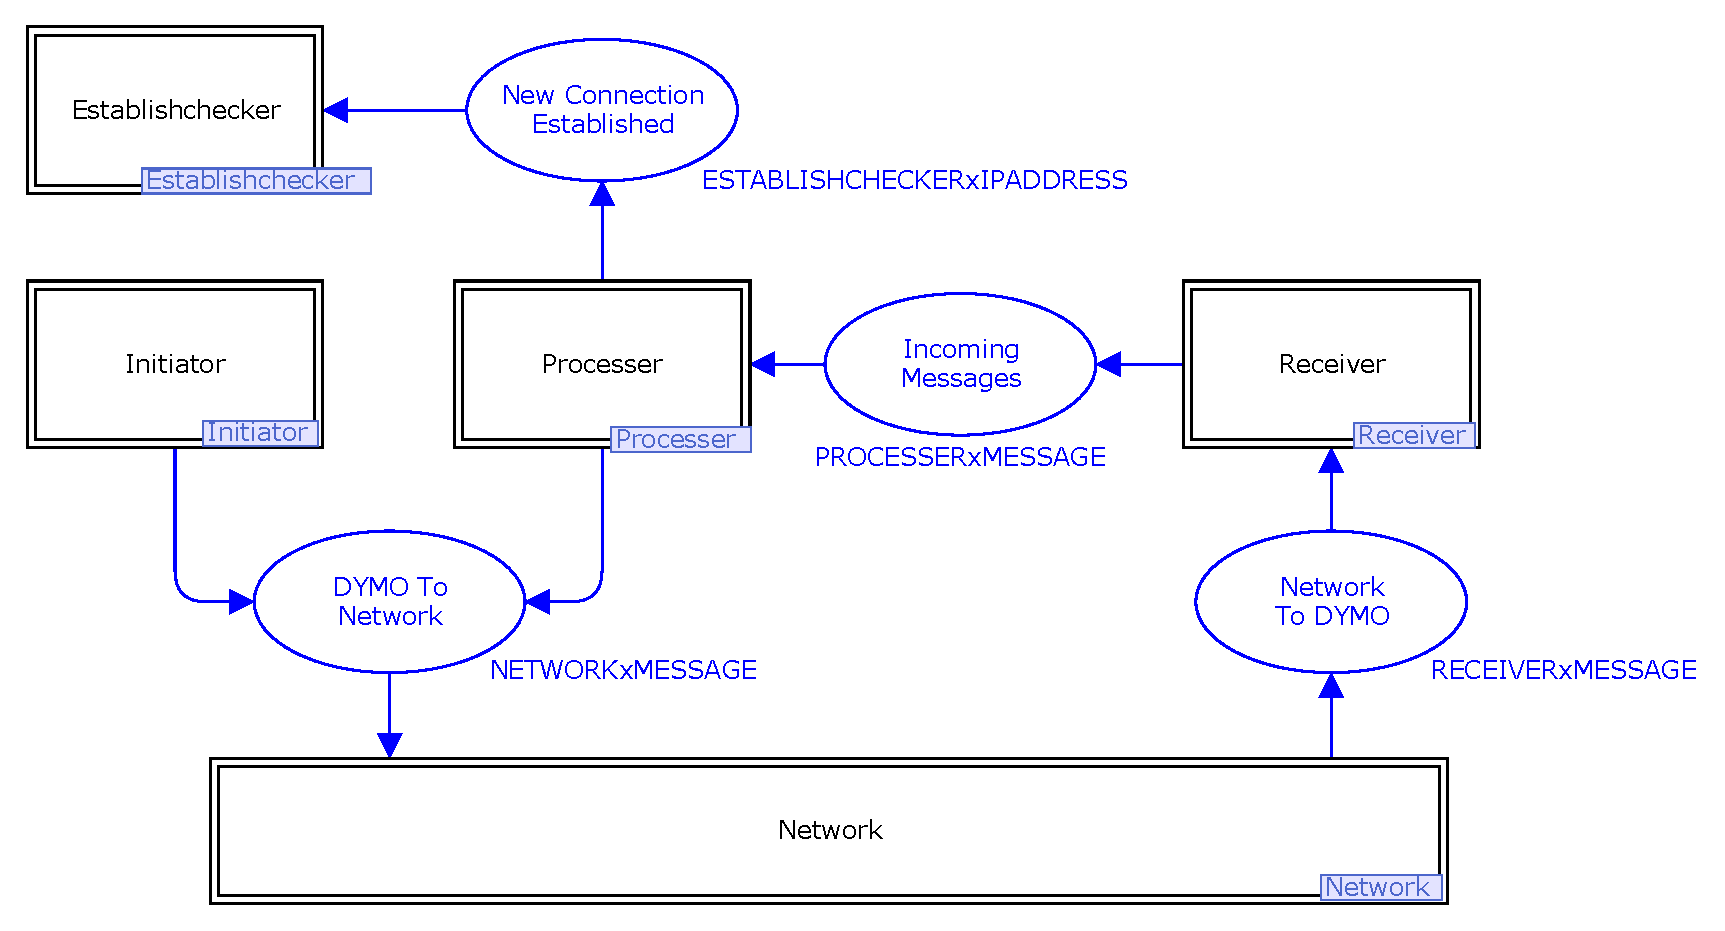
\includegraphics[width=\textwidth]{dymo/graphics/systemmodule.eps}
\caption{The \figitem{System} module of the ProPCPN DYMO model}
\label{fig:dymosystemmodule}
\end{figure}

Fig.~\ref{fig:dymosystemmodule} shows the prime (the root) module \figitem{System} of the ProPCPN DYMO model. The \figitem{System} module contains five \emph{substitution transitions} which are drawn as rectangular boxes with double lines. The substitution transitions are named \figitem{Establishchecker}, \figitem{Initiator}, \figitem{Network}, \figitem{Receiver}, and \figitem{Processer}. Each substitution transition is associated with a module which models the behaviour of the substitution transition. Tokens are exchanged between module using \emph{ports}. The ports constitutes the \emph{interface} of the module, i.e., a module can receive input via \emph{input ports}, and produce output via \emph{output ports}. In Fig.~\ref{fig:dymosystemmodule} all places are \emph{sockets}, i.e., places that are associated with an input or output port. The \figitem{System} module ties together the different parts of the protocol. The \figitem{Initiator} substitution transition creates new route requests. The \figitem{Establishchecker} substitution transition is responsible for notifying when a route has been established. The \figitem{Receiver} substitution transition judges the usefulness of the routing information found in received messages. The routing table is updated with the routing information if it is found useful. The messages that have not been discarded by the \figitem{Receiver} are send to the \figitem{Processer} that processes the messages depending on the message being a request or a reply. When the \figitem{Processer} has processed the message it can forward messages. The \figitem{Network} module is a simple reliable network. It forwards messages which is added to \figitem{DYMOToNetwork} and delivers it to the receiver by adding it to the place \figitem{NetworkToDYMO}.

\subsubsection{The Initiator Module}

\begin{figure}[b!]
\centering
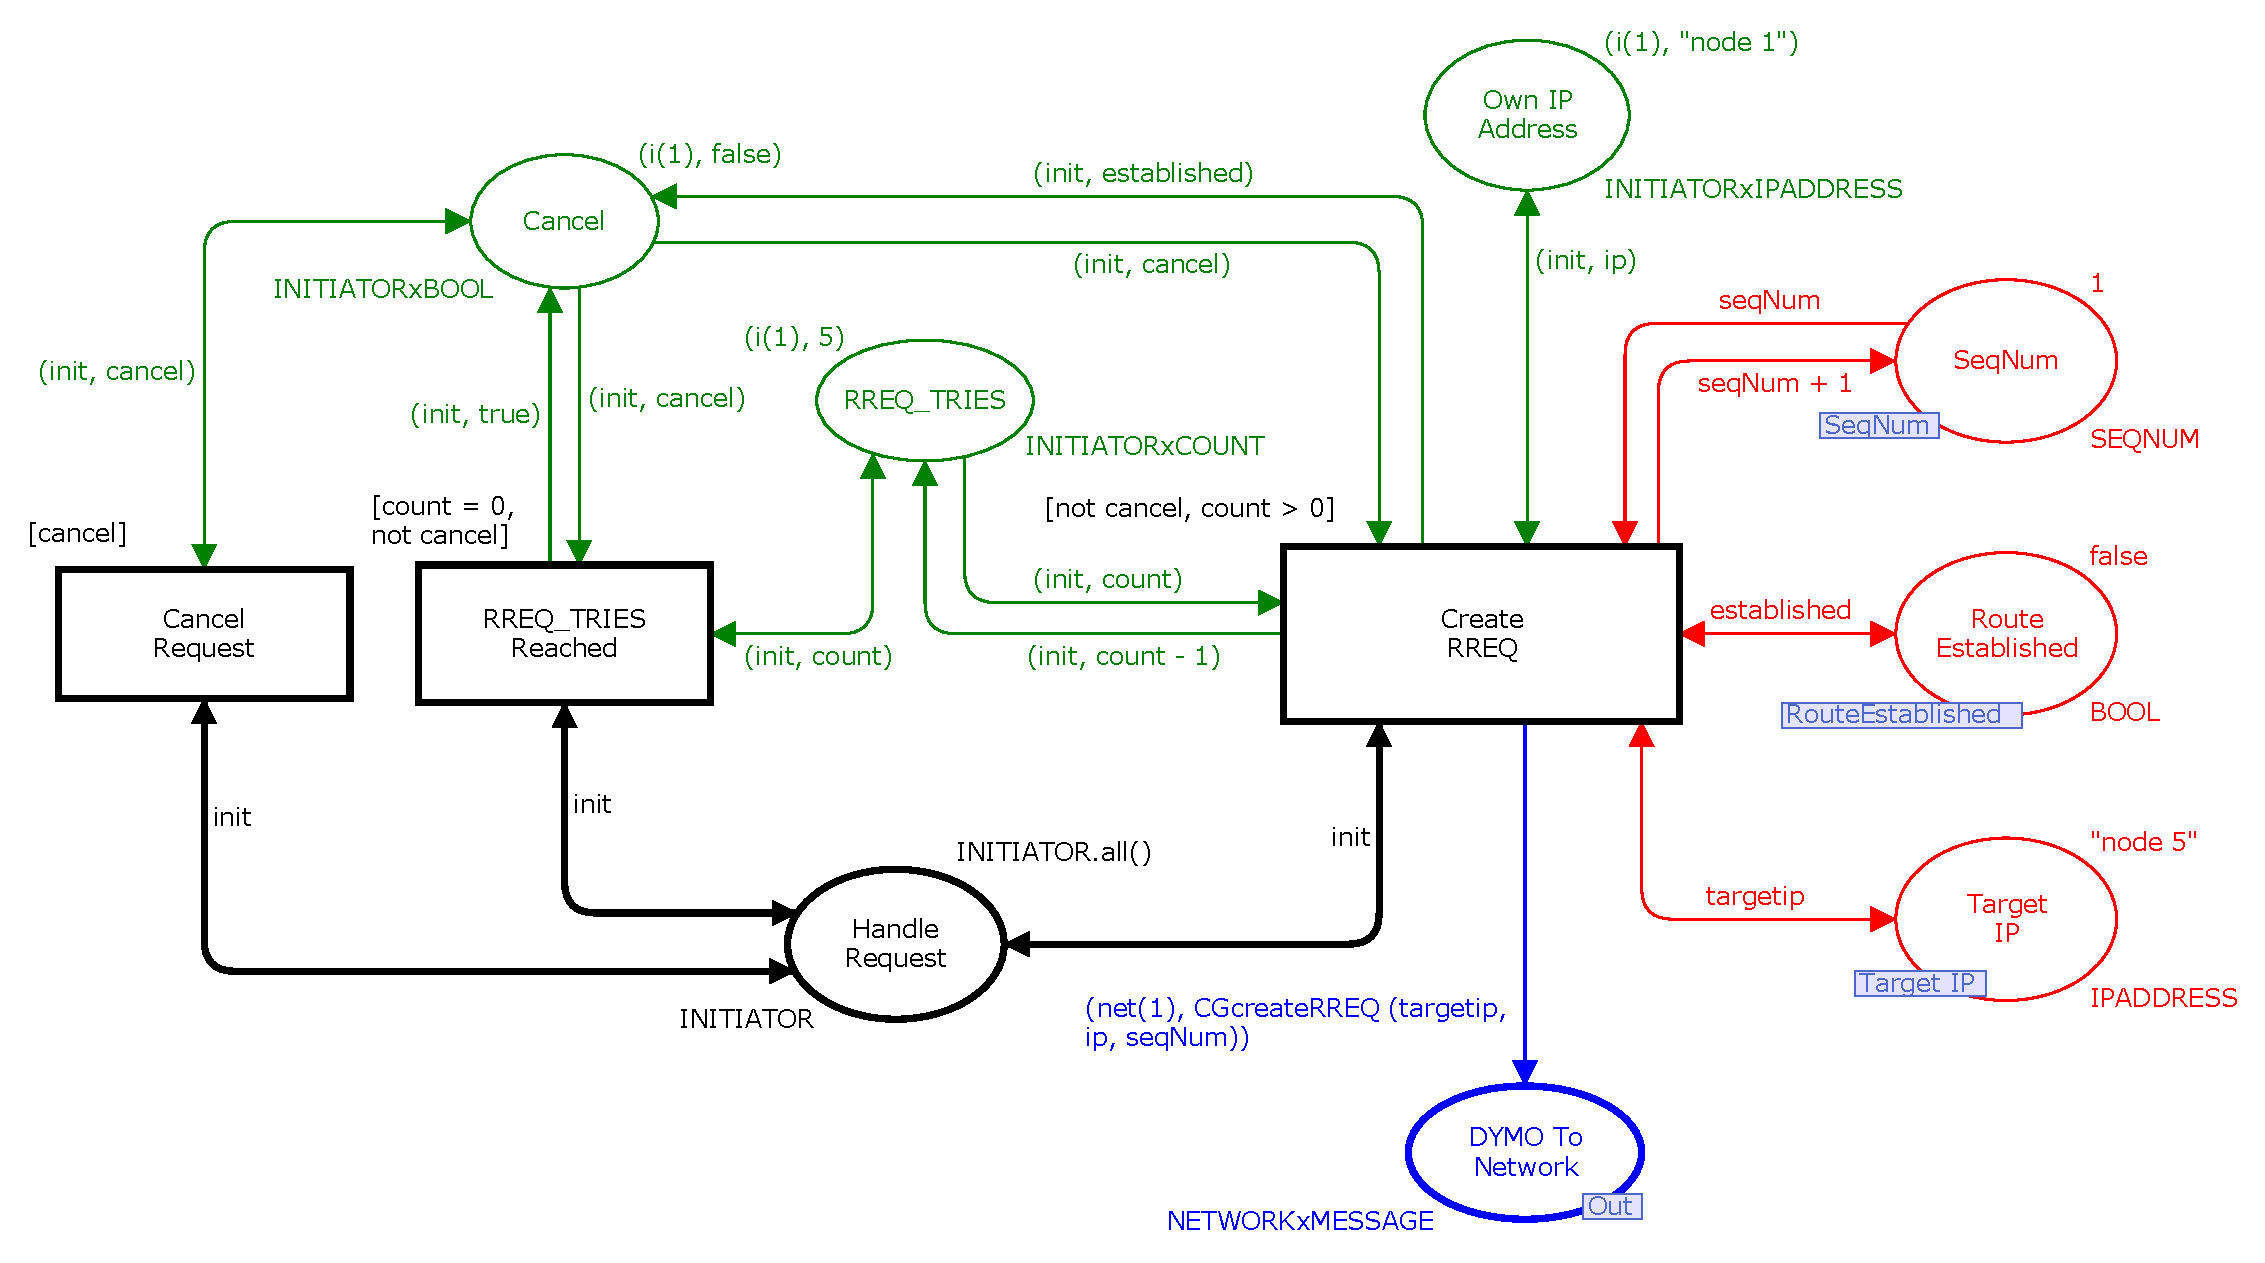
\includegraphics[width=\textwidth]{dymo/graphics/initiatormodule.eps}
\caption{The \figitem{Initiator} module of the ProPCPN DYMO model}
\label{fig:initiatormodule}
\end{figure}

Next, we take a closer look at the \figitem{Initiator} module shown in Fig.~\ref{fig:initiatormodule}. As mentioned this module is responsible for creating route request which is performed by the transition \figitem{CreateRREQ}. To create a route request the transition needs information about its own IP address, the target IP address, and the sequence number to put into the message. The IP address of a node is stored locally at the local place \figitem{OwnIPAddress}. The sequence number and the target IP address, is also used by the \figitem{Processer}, and is therefore modelled as shared places. To avoid too many arcs, which would make the model less readable, we have created shared places using \emph{fusion sets}. Places in different modules belonging to the same fusion set can be seen as one compound place, i.e., they always share the same marking, and they have the same colour set and initial marking.

The transition \figitem{CreateRREQ} do not produce route requests if a route already has been esbablished (determined by the shared place \figitem{RouteEstablished}), the retries limit has been reached (determined by the local place \figitem{RREQ\_TRIES}), or the request has been cancelled (determined by the local place \figitem{Cancel}). When a request has been made it is added to the buffer place \figitem{DYMOToNetwork}. This place has the \emph{output port tag} attached to show that it is an output port. As we saw in the \figitem{System} module in Fig.~\ref{fig:dymosystemmodule}, this place is assigned to a socket place with the same name connected to the \figitem{Network} substitution transition.

The other two transitions in the module handle the cancelation of requests. \figitem{RREQ\_TRIESReached} is enabled when the maximum number of retries has been reached, and it sets the value of the local place \figitem{Cancel} to true. When \figitem{Cancel} is true \figitem{CancelRequest} is enabled which means that no further action should be taken with this request.

\subsubsection{The Processer Module}
\begin{figure}
\centering
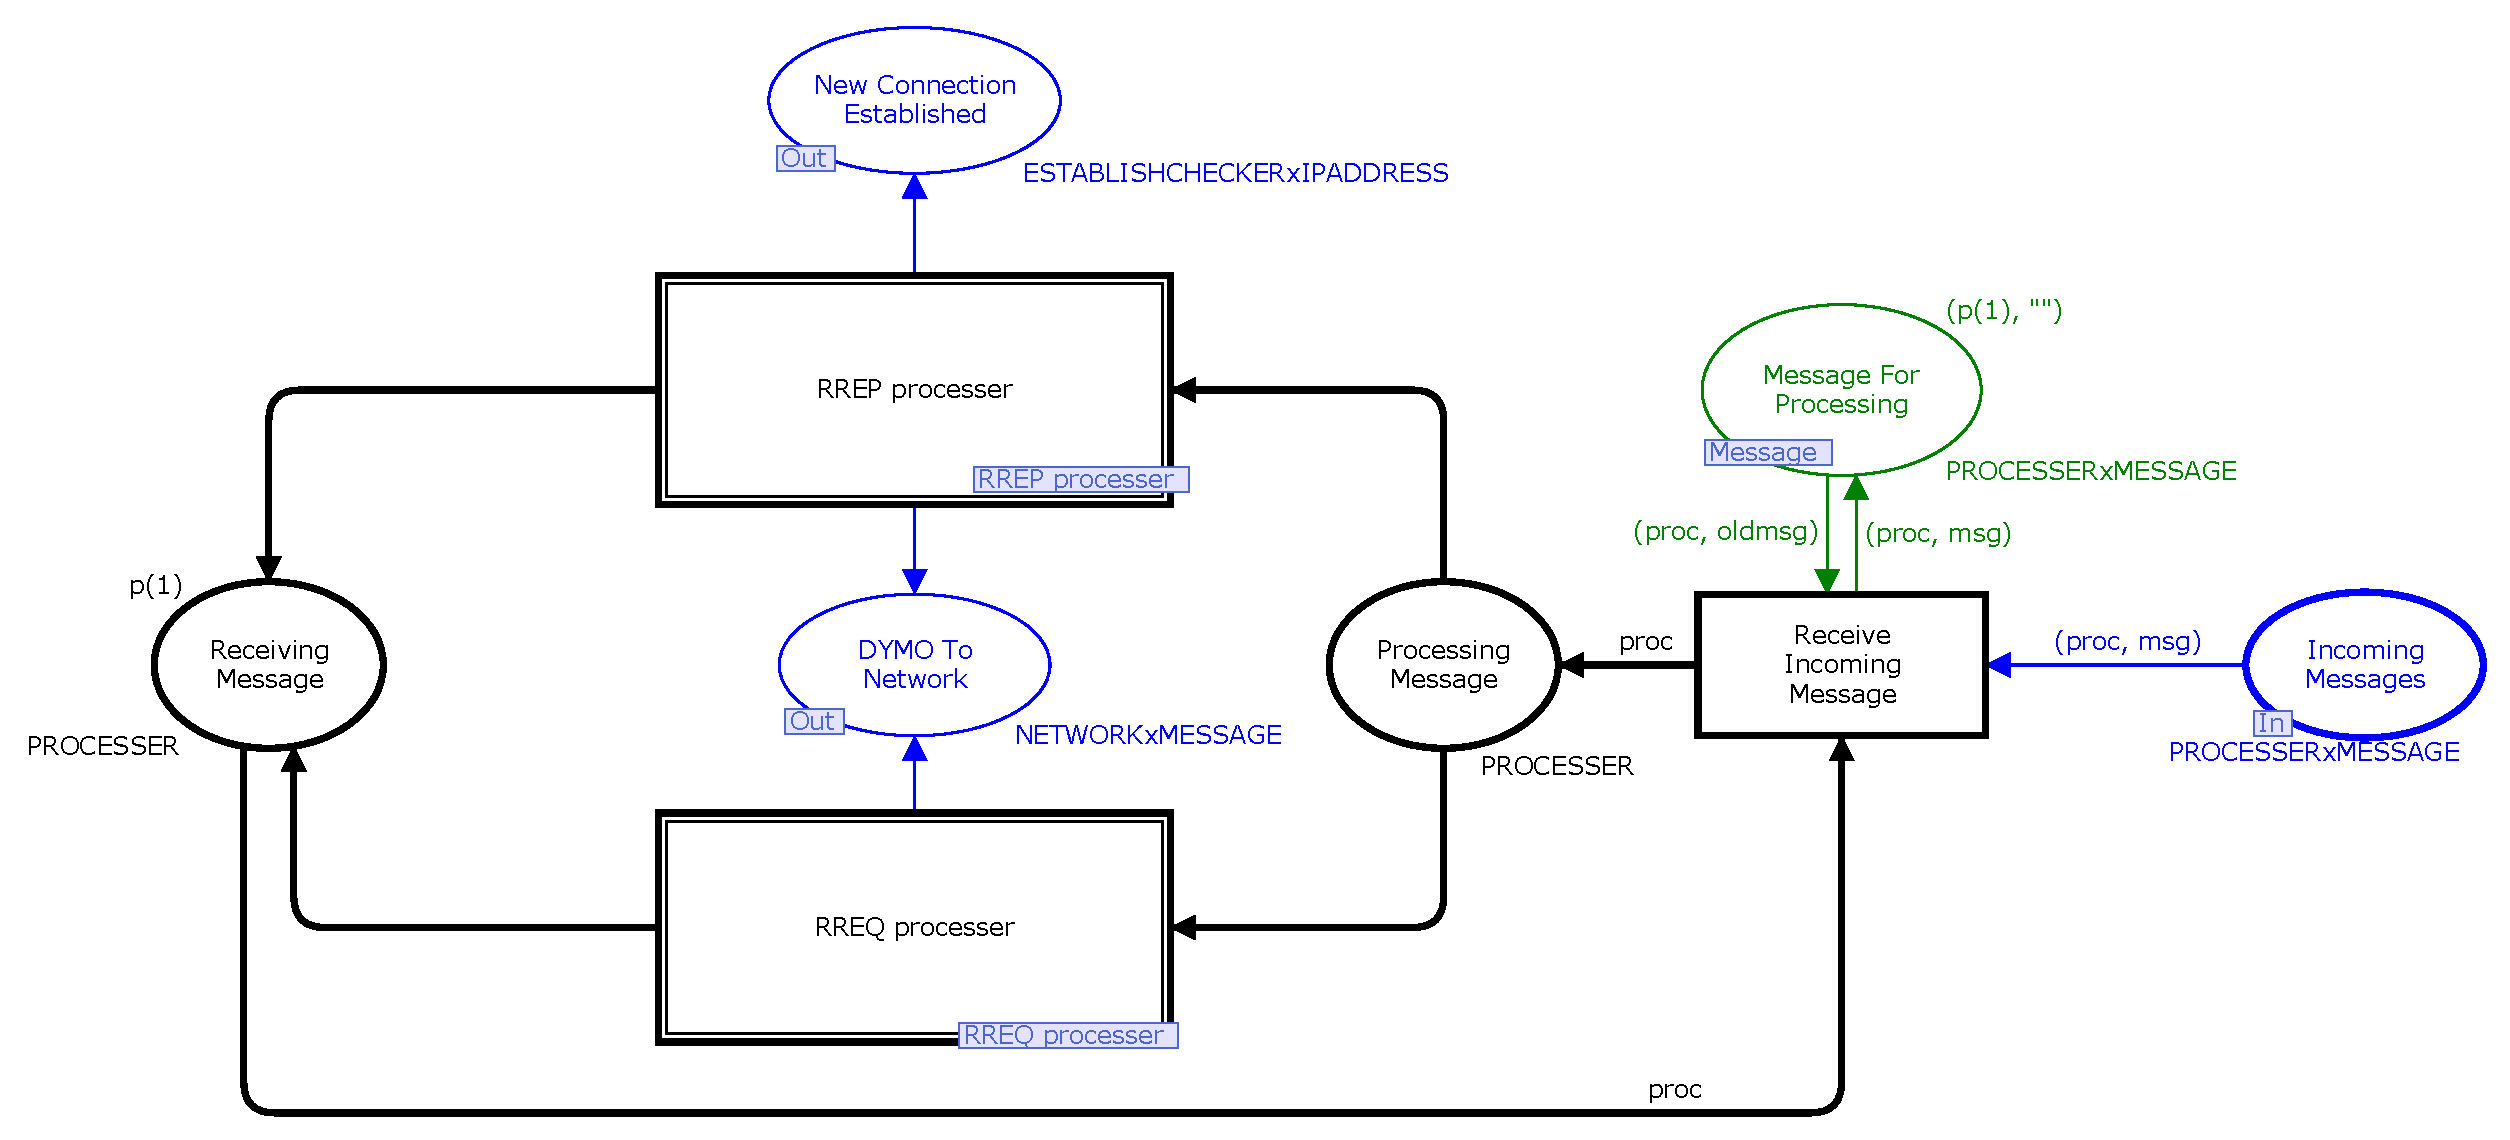
\includegraphics[width=\textwidth]{dymo/graphics/processermodule.eps}
\caption{The \figitem{Processer} module of the ProPCPN DYMO model}
\label{fig:processermodule}
\end{figure}

Moving on to Fig.~\ref{fig:processermodule} we find the \figitem{Processer} module. The \figitem{Processer} receives messages from the \figitem{Receiver} on the buffer place \figitem{IncomingMessages}. When a message arrives, the transition \figitem{ReceiveIncomingMessage} becomes enabled, and when it occurs the message is added to the local place \figitem{MessageForProcessing} for further processing. The process token is then added to the process place \figitem{ProcessingMessage}, and the control flow either continues to the substitution transition \figitem{RREPprocesser} or to the substitution transition \figitem{RREQprocesser} (depending on the type of the message).

\subsubsection{The RREPprocesser Module}
\begin{figure}
\centering
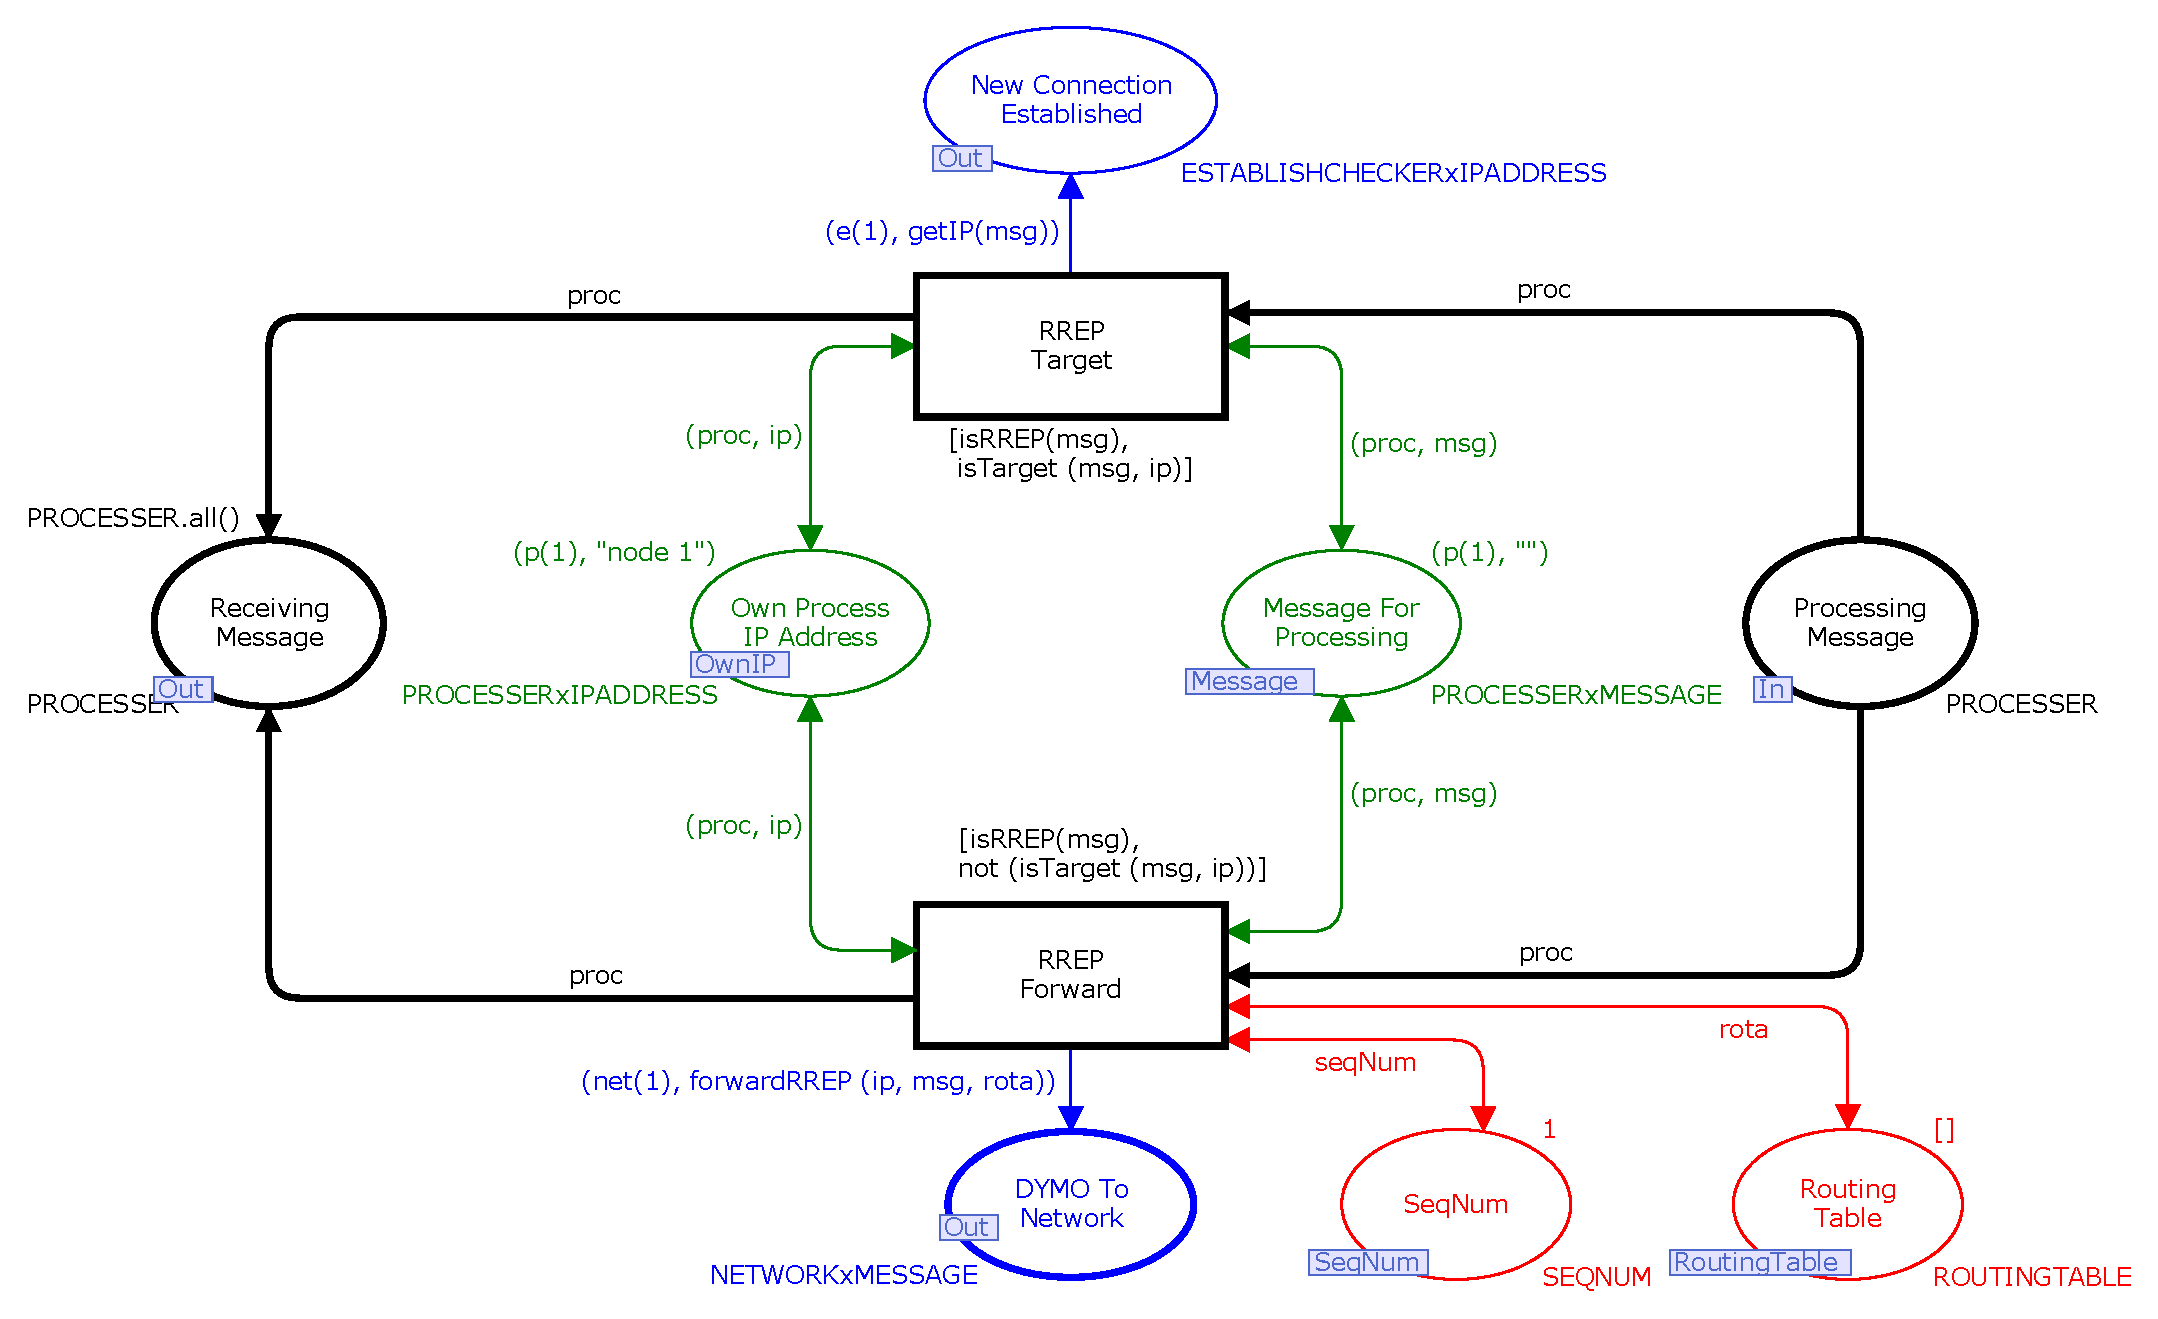
\includegraphics[width=\textwidth]{dymo/graphics/rrepprocessermodule.eps}
\caption{The \figitem{RREP processer} module of the ProPCPN DYMO model}
\label{fig:rrepprocessermodule}
\end{figure}

The \figitem{RREPprocesser} module (shown in Fig.~\ref{fig:rrepprocessermodule}) processes incoming messages which has the type RREP, i.e., a route reply. The messages are added to the local place \figitem{MessageForProcessing}, and if the current node is the target, the transition \figitem{RREPTarget} is enabled. An occurrence of \figitem{RREPTarget} means that the route has been established, and by adding the IP address of the originator of the RREP to the buffer place \figitem{NewConnectionEstablished} the \figitem{Establishchecker} is notified. If the current node is not the target of the RREP the transition \figitem{RREPForward} can occur. The transition \figitem{RREPForward} creates a new RREP message with the use of the shared place \figitem{SeqNum}, the shared place \figitem{RoutingTable}, and the local place \figitem{OwnProcessIPAddress}. The newly created message is added to the buffer place \figitem{DYMOToNetwork} and can then be transmitted over the network.
